% OB-SECTION {"id":"introduction","label":"sec-introduction","level":2,"order":1,"title":"Introduction"}

\section{Introduction}
\label{sec-introduction}
% OB-EDIT-BEGIN openbarry/markdown@1 id=introduction
Various approaches for adjusting the behaviors of large language models---including supervised finetuning~\cite{hu2022lora}, instruction tuning~\cite{wei2021flan}, and reinforcement learning from human feedback~\cite{christiano2017}---are widely used in practice~\cite{xia2024}.
Despite their effectiveness, these methods are costly, requiring specifically curated data and considerable computational resources.
Moreover, existing approaches do not use the fact that many existing models already exhibit desirable behaviors, instead opting to train in these behaviors from scratch.

\obtodo[id=cv-opening, created=2025-01-12T16:20:00.000Z, updated=2025-06-08T11:14:22.000Z, completed=2025-06-08T11:14:22.000Z]{Write the finetune-once, paste-many motivation and the three contributions.}

We propose \cmdv{}, an activation-based framework for transferring behaviors across models in a training-free way.
Specifically, we transfer adapter weights---parameter-efficient modules inserted into pretrained models---from a finetuned donor LLM to a recipient LLM via two main steps.
First, \cmdv{} identifies corresponding activation patterns between the donor and the recipient (Section~\ref{sec-method}).
Second, \cmdv{} derives a converter based on the donor's adapter weights, which facilitates inference with the recipient model.
These steps, which do not require additional data or training, result in improved downstream performance across several targeted tasks (Section~\ref{sec-experiments}).

\begin{figure}[t]
\centering
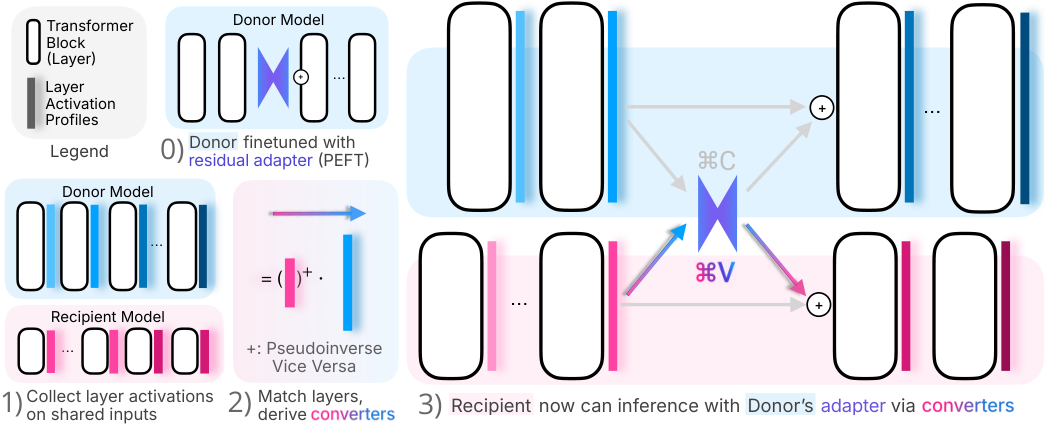
\includegraphics[width=0.99\linewidth]{figures/overview2.png}
\caption{Reusing PEFT weights on an architecturally different model with \cmdv{} requires little data and no backpropagation.
\cmdv{} can bring recipient models behaviors like jailbreaking prompt refusal.}
\label{fig:pipeline}
\end{figure}

Our contributions:
\begin{enumerate}
\item \textbf{Activation profiling.} A data-efficient method that establishes correspondences between residual neurons in distinct transformer LLMs.
\item \textbf{\cmdv{} adapter transfer.} Using activation profiles, we derive converters that paste new behaviors into a recipient without additional data or parameter updates.
\item \textbf{Effective behavior pasting.} On safety refusal, jailbreaking, and chain-of-thought prompting, \cmdv{} matches finetuning while using minimal compute.
\end{enumerate}

\obclaim{\cmdv{} matches or exceeds direct DiReFT on refusal, jailbreak, and auto-CoT while deriving converters in 6.35s on a laptop CPU and without the original training data.}
% OB-EDIT-END id=introduction
